\section{The main update and a packing bound for secondary seeds}
\label{main:section}

This section gives system $A$ its two separation mechanisms and extracts
the geometric information available when both fail. Main clipping either
separates a pair or supplies short descending paths at its endpoints. A
low separating tip supplies a component certificate. The remaining
endpoints satisfy a packing bound that lets one secondary proposal act
alone with positive probability and bounds the number of formulas
competing near a point.

All lengths in this section are measured in the units of the current
scale.  Thus the pairs under consideration satisfy
$1\le d(x,y)\le2$.  We use the parameters and the random bands of
Sections~\ref{sets:parameters} and~\ref{sets:setup}.  In particular,
$J_2\subset J_1$ denotes a narrow band contained in its broad band.
The cells used below are the connected column cells of
Lemma~\ref{geo:cells}.  The frontier of a cell $C$ is the union, within
$J_1$, of all its column intervals whose columns have an active link
to a column outside $C$.  When two cells have a common quotient point,
that point is in the frontier of both cells.  Frontier values will
therefore always be left unchanged.

An ordinary chart of system A has field $P=C_0+\tau s$, where
$\tau\in\{-1,1\}$ and $s=d_I(o,\cdot)$ on a component of an old band
$I$, or $s=0$ in the constant case.  Within that chart we perform all
comparisons in the $s$ orientation.  Replacing $s$ by $s'$ means
replacing $P$ by $C_0+\tau s'$ in the original label variables.

\subsection{The main update}
\label{main:update-section}

Let $C$ be a cell of width $D$ in $J_1$.  We make it available for an
update only when its entire closed $d$-neighborhood of radius $1$
is contained in one old ordinary chart of system A.  This condition
allows every path of length at most $10D$ starting in $C$ to be
evaluated in that chart: all its points are in the indicated
neighborhood, and hence in the band component on which the old field
is defined.  In particular,
\begin{equation}
 |s(v)-s(w)|\le d_{J_1}(v,w)\le10D
 \qquad(v,w\in C).
 \label{main:cell-field-variation}
\end{equation}
Here and below an intrinsic shortest path of length at most $10D$
is allowed to leave the cell.  Its length bound, rather than intrinsic
connectedness of the cell, ensures its availability in the old chart.

The frontier bounds how far a strictly Lipschitz proposal can rise at an
interior point. If a frontier constraint prevents a definite rise, a
shortest path to that constraint will be almost maximally descending
for the old field. A downward shift makes the proposal strictly inactive
at the frontier, which will also protect small balls crossing cell boundaries.

Fix $v_C\in C$ and put $s_C=s(v_C)$.  On the entire $J_1$-component
containing $C$, define
\begin{equation}
 p_C(v)=\min\left\{s_C+1,
       \inf_{z\in\partial C}
       \bigl(s(z)+(1-\zeta_A)d_{J_1}(v,z)\bigr)\right\}.
 \label{main:frontier-extension}
\end{equation}
The infimum over an empty frontier is $+\infty$.  The frontier is a
finite union of compact column intervals, so that a finite infimum
is attained.  The function $p_C$ is $(1-\zeta_A)$-Lipschitz for
$d_{J_1}$.  Apply Theorem~\ref{int:interpolation}, with error $E_A$,
to obtain $\widetilde p_C$, and set
\begin{equation}
 F_C=\widetilde p_C-4E_A.
 \label{main:F}
\end{equation}
In particular,
\begin{equation}
 p_C-5E_A\le F_C\le p_C-3E_A.
 \label{main:F-error}
\end{equation}

For a fresh offset $\alpha_C\in[0,E_A]$, define a function of height
$p_{h,C}$ as follows.  It is $s_C-1+\alpha_C$ at either endpoint of
$J_1$, is $s_C+2+\alpha_C$ on the interval obtained by deleting
the outer portions of width $0.09a_1$, and is linear on the two
remaining portions.  Extend it constantly beyond the two endpoints
of $J_1$.  Its Lipschitz constant is $3/(0.09a_1)$.
If the independent fair coin of $C$ is kept, make the replacement
\begin{equation}
 s'(v)=\max\{s(v),\min\{F_C(v),p_{h,C}(h(v))\}\}
 \qquad(v\in C).
 \label{main:replacement}
\end{equation}
Otherwise leave the cell unchanged.  Cells that are unavailable
are also left unchanged.

\begin{lemma}[Validity and size of the main replacement]
\label{main:validity}
The simultaneous replacements~\eqref{main:replacement} respect
switches, preserve vertical nesting and the vertical upper bound
for system A, and admit ordinary charts on every new branch.
At any point the change in the system-A label set has measure at most
$\kappa_A(1+10D)$.
\end{lemma}

\begin{proof}
At a frontier point $z$, the term with source $z$ in
\eqref{main:frontier-extension} gives $p_C(z)\le s(z)$.  Thus
$F_C(z)\le s(z)-3E_A$.  At either endpoint of the height band,
\eqref{main:cell-field-variation} gives
\[
 p_{h,C}\le s-1+10D+E_A<s.
\]
The replacement therefore equals the old field on every frontier
and at every height endpoint, with a strict margin in the proposed
branch.  Different cell prescriptions agree at common quotient
points.  Within a cell, every constituent respects switches.

The old field and $F_C$ have vertical Lipschitz constant at most $1$;
the height branch has constant $3/(0.09a_1)$.  The maximum and minimum
in~\eqref{main:replacement} have the maximum of these constants.
The parameter choice makes its product with $\kappa_A$ strictly
less than $1$.  The vertical replacement and gluing rule for label
sets consequently preserves nesting and the vertical upper bound.

An unchanged branch keeps its old ordinary chart.  A winning atom
of $F_C$ has the form $c\pm d_{J_1}(k,\cdot)$ and therefore gives
an ordinary chart after converting back from the $s$ orientation.
A winning height branch is recorded by the height-only change of
variables from the label-set construction, with a fresh constant
chart.  Identifiers can be chosen using the update data and the
winning atom, with the inherited identifier retained wherever the
old field wins.

Finally, the replacement never decreases $s$, and
\[
 F_C\le s_C+1-3E_A\le s+1+10D.
\]
Consequently $0\le s'-s\le1+10D$.  At a fixed point, a change
$s'-s$ in the common chart changes the label set by measure
$\kappa_A|s'-s|$, which proves the stated bound.
\end{proof}

\begin{definition}[Descending path]
\label{main:ray-definition}
A descending path at a point $w$ is a shortest path in $J_1$, of
length $d_0\in[10^{-5},0.02]$, whose terminal point $z$ satisfies
\begin{equation}
 s(z)\le s(w)-d_0+\epsilon.
 \label{main:ray-endpoint}
\end{equation}
It is parametrized by arclength $t\in[0,d_0]$.  All descending paths
used below lie in the old ordinary chart band, so $s$ can be
evaluated at every point of the path.
\end{definition}

\begin{lemma}[Main raise or a descending path]
\label{main:ray}
Suppose $w$ satisfies the height and radial interior requirements
for its width-$D$ cell, and that the cell is available.  For every
choice of the interpolation parameters, its kept replacement
raises $s(w)$ by more than $2E_A$, unless a descending path at $w$
exists.  Every descending path satisfies
\begin{equation}
 s(\gamma(t))\le s(w)-t+\epsilon
 \qquad(0\le t\le d_0).
 \label{main:ray-prefix}
\end{equation}
\end{lemma}

\begin{proof}
Assume that the raise is at most $2E_A$.  The height interior
requirement places $w$ on the plateau of $p_{h,C}$, where
\[
 p_{h,C}(h(w))\ge s(w)+2-10D>s(w)+2E_A.
\]
It follows that $F_C(w)\le s(w)+2E_A$, and
\eqref{main:F-error} then gives
\begin{equation}
 p_C(w)\le s(w)+7E_A.
 \label{main:small-extension}
\end{equation}
The constant branch $s_C+1$ is strictly greater than the right-hand
side of~\eqref{main:small-extension}.  The frontier is therefore
nonempty, and there is a minimizing $z\in\partial C$ with
\[
 s(z)+(1-\zeta_A)d_{J_1}(w,z)\le s(w)+7E_A.
\]
Put $d_0=d_{J_1}(w,z)$.  The radial padding conclusion of
Lemma~\ref{geo:padding} gives $d_0\ge0.01D=10^{-5}$.
The weak diameter estimate gives $d_0\le10D<0.02$.
Choose an intrinsic shortest path from $w$ to $z$.  It remains in
the old chart band by availability.  Since
\[
 \zeta_A d_0+7E_A
 \le (\epsilon/100)(10D)+7\epsilon/1000<\epsilon,
\]
this path satisfies~\eqref{main:ray-endpoint}.

For the last assertion, apply the old field's Lipschitz bound to
the remaining subpath, of length $d_0-t$:
\[
 s(\gamma(t))\le s(z)+(d_0-t)
                 \le s(w)-t+\epsilon.
\]
\end{proof}

\begin{corollary}[Separation supplied by the main test]
\label{main:pair-separation}
Let $(x,y)$ be an eligible pair satisfying the interior requirements,
$1\le d(x,y)\le2$, and $|s(x)-s(y)|\le E_A$.  If either endpoint
has no descending path, then, conditional on main-update mode,
the independent cell coins give probability at least $1/4$ of
system-A symmetric-difference separation at least $\kappa_A E_A$
at this step.
\end{corollary}

\begin{proof}
The two endpoints lie in different width-$D$ cells, since a cell
has $d$-diameter at most $10D<1$.  Each of these cells is available:
its radius-$1$ neighborhood lies in the radius-$5$ neighborhood
of its endpoint, by the cell diameter bound and eligibility.
Keep the coin at an endpoint with no descending path and suppress
the coin of the other endpoint.  This has probability $1/4$.
Lemma~\ref{main:ray} raises the first comparison value by more
than $2E_A$ and leaves the second unchanged, so their new field
difference has magnitude at least $E_A$.  Evaluate both new sets
in their common old label variables.  The common-chart
symmetric-difference formula gives the asserted bound.
\end{proof}

\subsection{The component barrier and the seed set}
\label{pack:seed-definition-section}

The main test has reduced the problem to pairs with two descending paths.
Before using those paths to locate nearby groups, we remove pairs already
separated by a low terminal tip. The resulting certificate records only
three memberships, so later changes elsewhere cannot invalidate it.

For the rest of the section, retain only eligible pairs $(x,y)$ in
the distance range $[1,2]$ that satisfy all the interior requirements
and both field-difference cutoffs, lie in the same bands $J_2\subset
J_1$, and possess descending paths at both endpoints.  In particular,
their common ordinary system-A field $s$ is nonconstant: a constant
field cannot satisfy~\eqref{main:ray-endpoint} with
$d_0\ge10^{-5}>\epsilon$.
Choose once and for all a representative column for every vertex
under consideration.  A chord separates two representatives
strictly if they lie in the strict interiors of the two complementary
circular arcs determined by its endpoint columns.

\begin{lemma}[Label mass at a separating tip]
\label{pack:barrier}
Suppose a retained pair has a non-neighbor link separating its
representatives strictly, with tip $e$ at a height in $J_2$, such
that $d(e,x)\le1$ or $d(e,y)\le1$.  If
\begin{equation}
 s(e)<s(w)-j
 \label{pack:drop}
\end{equation}
for at least one endpoint $w$, then there is label mass at least
$\kappa_Aj/4$ for which both endpoints are active and $e$ is
inactive.  In no-change mode this gives a component-refined
separation in system A of at least $\kappa_Aj/2$ at this step.

More generally, suppose subsequent changes have total unrefined
symmetric-difference costs $\Delta_x,\Delta_y,\Delta_e$ at the
three points.  The final component-refined separation is at least
\begin{equation}
 2\bigl(\kappa_Aj/4-\Delta_x-\Delta_y-\Delta_e\bigr)_+.
 \label{pack:barrier-damage}
\end{equation}
\end{lemma}

\begin{proof}
Eligibility puts $x,y,e$ in the same old ordinary chart.  Write
$P=C_0+\tau s$ there and restrict labels to the sign $\sigma=\tau$.
On this half of the label space the threshold at $v$ is
\[
 T_v=h(v)+\kappa_A\tau C_0+\kappa_As(v).
\]
The other endpoint has $s$-value within $E_A$ of $s(w)$.
Also all three heights lie in $J_2$.  Thus, for $v=x,y$,
\[
 T_v-T_e\ge\kappa_A(j-E_A)-a_2\ge\kappa_Aj/2,
\]
using $E_A\le j/4$ and $a_2\le\kappa_Aj/4$.
The labels with $\sigma=\tau$ and
$T_e\le Z<\min\{T_x,T_y\}$ have the required three membership
conditions and mass at least $\kappa_Aj/4$.  Choices at the
threshold endpoints have measure zero.

Lemma~\ref{sets:component-refinement} separates the two active
points into different components whenever the tip is inactive;
each such label contributes $2$ to the refined distance.
After later changes, the subset of this label mass on which any
of the three memberships changes has measure at most
$\Delta_x+\Delta_y+\Delta_e$.  Apply the same component-refinement
lemma to the surviving labels in the final nested system.  This
proves~\eqref{pack:barrier-damage}; no control of the changes in
component names is required.
\end{proof}

Exclude every retained pair to which Lemma~\ref{pack:barrier}
applies.  The secondary seed set consists of all endpoints of the
remaining pairs.  If a vertex occurs in several remaining pairs,
regard it as one seed and fix one of those pairs as its witness;
write $w'$ for its witness partner.  Fix descending paths for both
members of each chosen witness pair.  All these choices are made
from the old fields and bands, before any secondary interpolation
noises are sampled.

Group seeds by their broad and narrow bands, their width-$g$ cell
in the broad band, and their old chart identifiers in both systems.
The groups are used only to organize the update.  They introduce
no new chart boundaries.  By the weak cell diameter bound, two
seeds in the same group have $d_{J_1}$-distance at most $10g$;
a shortest path of this length is in their common old chart bands
by eligibility.  Their ordinary fields consequently vary by at most $10g$. The full
system-$B$ fields vary by at most $50g$, since their old-chart Lipschitz
constants are less than $5$.

\subsection{Packing the groups that meet a narrow-band ball}
\label{pack:section}

We put the relevant seeds in one circular gap of a connected low sublevel
set. Two paths to extreme seed indices then visit or skip every seed
column. A skipped seed must descend toward an endpoint of the skipping
link. Since its pair survived the low-tip test, that endpoint cannot be
much lower than the seed, so the descent reaches it quickly. All selected
seeds are consequently close to two short paths, where padding bounds
their number.

\begin{proposition}[Restricted packing bound]
\label{pack:bound}
Fix a narrow band $J_2$.  In any component of $X_{J_2}$, every
closed $d_{J_2}$-ball of radius $4R$ meets seeds from at most
\begin{equation}
 M_{\mathrm{pack}}=2+\left\lceil1600R/g\right\rceil
 \label{pack:number}
\end{equation}
groups.  This bound is independent of the graph, the number of
columns, and the history of the construction.
\end{proposition}

\begin{proof}
Let $B$ be such a ball, with arbitrary center $z$.  If it has no
seeds there is nothing to prove.  Otherwise fix $w_*\in B$ among
the seeds.  Only a narrow band contained in a broad band can have
seeds.  Its broad band $J_1$ is then unique, and the $J_2$-paths
from $z$ to the seeds show that all of them lie in one
$J_1$-component.

All seeds of $B$ have the same chart identifier in either system.
Indeed $d(z,w)\le4R<5$ for every such seed $w$, so $z$ lies in
the common chart of its eligible witness pair.  Since charts
partition $X$, those identifiers coincide.  Write $I$ for their
common old system-A band and $s=d_I(o,\cdot)$ for its distance
field.  All center-to-seed paths of length at most $4R$, all
descending witness paths, and the vertical intervals used below
are contained in the relevant old chart band: they are at distance
less than $5$ from an endpoint of an eligible witness pair.
For example, a point on a center-to-seed path has distance at most
$8R$ from $w_*$, and a descending path has length at most $0.02$.
The additional vertical intervals have length at most $a_1$.
In particular $J_1\subset I$ as height intervals: the full column
interval $J_1$ through any seed is within its radius-$5$
neighborhood.

Set $H=h(w_*)$ and form the profile $q_i=s(i,H)$, with $+\infty$
outside the old component as in Lemma~\ref{geo:sublevel}.  Put
\begin{equation}
 t=s(w_*)-\tfrac12\,10^{-5},\qquad S=\{i:q_i\le t\}.
 \label{pack:low-set}
\end{equation}
For every seed $w\in B$, the path through $z$ gives
\[
 |s(w)-s(w_*)|\le8R,
 \qquad |s(w')-s(w)|\le E_A.
\]
The terminal column $i$ of either chosen descending path for
$(w,w')$ therefore satisfies
\[
 q_i\le s(w_*)+8R+E_A-10^{-5}+\epsilon+a_1<t,
\]
where we used
$8R+E_A+\epsilon+a_1<\tfrac12\,10^{-5}$.
Thus $S$ is nonempty, and it is connected in the active graph
of $I$ by Lemma~\ref{geo:sublevel}.

Every column on any center-to-seed path of length at most $4R$
lies outside $S$.  In fact, if such a path visits column $i$ at
point $v$, then
\[
 q_i\ge s(v)-a_1\ge s(w_*)-8R-a_1>t.
\]
All comparisons take place in $I$, as verified above.  The
noncrossing gap property, Lemma~\ref{geo:gap}, now places all
these path words and their endpoint representatives in one
linear circular gap of $S$.  Fix a representative of $z$ to
order this gap.  Equivalent representatives also lie in the
same gap, since a zero-length switch path satisfies the same
avoidance argument.

Choose one representative seed from each group meeting $B$.
In the linear order of the gap, choose a seed of minimum index
among those to the left of the center index, if there is one,
and similarly a seed of maximum index on the right.  Let
$P_-$ and $P_+$ be shortest $J_2$-paths from $z$ to these extreme
seeds.  When one side has no seed, use the constant path at $z$
on that side.  Each path has length at most $4R$.
For any chosen seed $w$, at least one of these two path words
either visits its representative column or makes a switch
strictly over its index.  This is the elementary skipping
property of Lemma~\ref{geo:skipping}, applied between the
center and the extreme index on that side.

If the path visits the column of $w$, a vertical interval of
length at most $a_1$ connects $w$ to a point of that path in
$J_1$.  Consider instead a switch strictly over its index.
Let $a,b$ be the switching columns, ordered within the gap so
that the representative of $w$ is in $(a,b)$.  The switch is
not a circular-neighbor link, because its strict interval
within the gap contains a column and the complementary arc
contains the nonempty set $S$.  It is consequently a single
switch at a tip $e$, by the column-model hypothesis.  This tip
is on $P_-$ or $P_+$, has height in $J_2$, and satisfies
\begin{equation}
 d(w,e)\le8R<1.
 \label{pack:tip-near}
\end{equation}
The interval $(a,b)$ is disjoint from $S$.

We claim that the witness partner $w'$ has representative
strictly outside the closed interval $[a,b]$ in the circle.
If its representative were in $(a,b)$, its descending path,
whose terminal column belongs to $S$, would have to visit
column $a$ or $b$.  This follows from noncrossing, or directly
from Lemma~\ref{geo:chord-separation}.  Join that visit
vertically to $e$, then follow the appropriate extreme path
back to $z$ and a shortest center-to-$w$ path.  The resulting
path has length at most
\[
 0.02+a_1+8R<1,
\]
contradicting $d(w,w')\ge1$.  If $w'$ itself has representative
$a$ or $b$, the vertical connection to $e$ gives the same
contradiction without the descending segment.  This proves
the claim.

The link at $e$ thus separates the two witness representatives
strictly.  Because the witness pair was not excluded and
\eqref{pack:tip-near} holds, its failure to satisfy the
barrier-drop condition implies
\begin{equation}
 s(e)\ge s(w)-j.
 \label{pack:tip-not-low}
\end{equation}
The descending path from $w$ must likewise hit column $a$ or
$b$, since it begins in $(a,b)$ and ends in $S$.  Let $v$ be
its first such hit and let $p$ be the arclength to $v$.
Lemma~\ref{main:ray} and the vertical comparison with $e$ give
\[
 s(v)\le s(w)-p+\epsilon,
 \qquad
 s(v)\ge s(e)-a_1\ge s(w)-j-a_1.
\]
It follows that $p\le j+\epsilon+a_1$.  The descending prefix
and the vertical interval from $v$ to $e$ both lie in $J_1$,
so
\begin{equation}
 d_{J_1}(w,e)\le j+\epsilon+2a_1.
 \label{pack:near-path}
\end{equation}

We have proved that every chosen seed is within
$\rho_{\mathrm{pack}}=j+\epsilon+2a_1$ in $d_{J_1}$ of
$P_-\cup P_+$.  Distinct chosen groups have distinct width-$g$
cells: their bands, band component, and two old identifiers
have already been shown to coincide.  Their seed points are
radially padded, so Lemma~\ref{geo:padding} gives pairwise
$d_{J_1}$-separation at least $b_0=0.01g$.

For each chosen seed, take one of the path points just
constructed within $\rho_{\mathrm{pack}}$, and assign it to one path
containing it.  Path points assigned to different seeds have
$d_{J_1}$-distance at least $b_0-2\rho_{\mathrm{pack}}\ge b_0/2$.
Their arclength parameters on either path are therefore
separated by at least $b_0/2$.  A path of length $4R$ has at
most $1+8R/b_0$ such points.  The two paths together have at
most
\[
 2+16R/b_0=2+1600R/g
\]
assigned points.  This proves~\eqref{pack:number}.
\end{proof}

Figure~\ref{fig:surviving-seeds} shows the skipping-link argument and the
short descending prefix that places a surviving seed near an extreme path.

\begin{figure}[tbp]
\centering
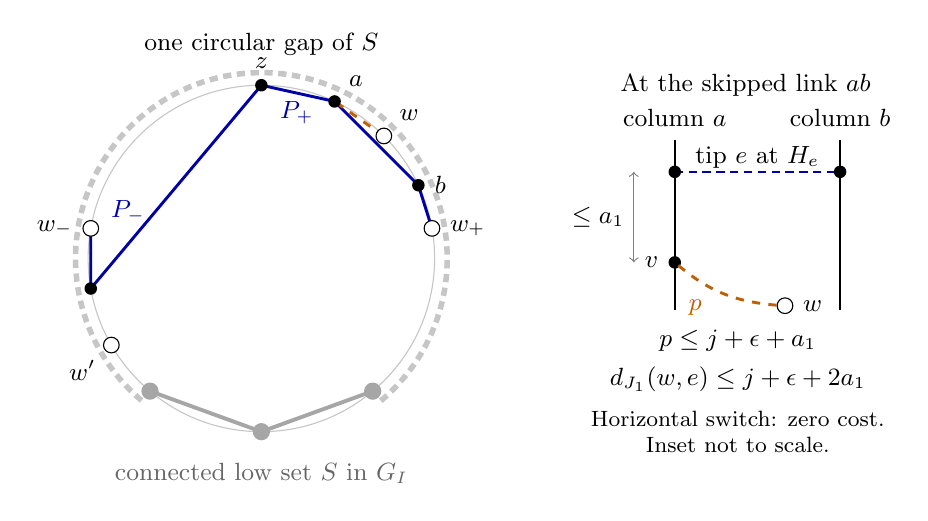
\begin{tikzpicture}[x=1cm,y=1cm,font=\small,
  vertex/.style={circle,fill=black,inner sep=1.6pt},
  seed/.style={circle,draw=black,fill=white,inner sep=2pt},
  low/.style={circle,fill=gray!70,inner sep=2.2pt}]
  \draw[gray!45] (0,0) circle (2.2);
  \draw[gray!45,densely dashed,line width=2pt] (310:2.36) arc (310:590:2.36);
  \node[align=center,fill=white,inner sep=2pt] at (0,2.72) {one circular gap of $S$};
  \coordinate (z) at (90:2.2);
  \coordinate (wm) at (170:2.2);
  \coordinate (q) at (190:2.2);
  \coordinate (wp) at (10:2.2);
  \coordinate (a) at (65:2.2);
  \coordinate (b) at (25:2.2);
  \coordinate (w) at (45:2.2);
  \coordinate (partner) at (210:2.2);
  \coordinate (s1) at (230:2.2);
  \coordinate (s2) at (270:2.2);
  \coordinate (s3) at (310:2.2);
  \draw[gray!70,line width=1.4pt] (s1)--(s2)--(s3);
  \draw[blue!65!black,line width=1.05pt] (z)--node[left,pos=.62] {$P_-$} (q)--(wm);
  \draw[blue!65!black,line width=1.05pt] (z)--(a)--(b)--(wp);
  \node[blue!65!black] at (.45,1.85) {$P_+$};
  \draw[orange!75!black,dashed,line width=1.05pt] (w)--(a);
  \node[vertex,label=above:$z$] at (z) {};
  \node[seed,label=left:$w_-$] at (wm) {};
  \node[vertex] at (q) {};
  \node[seed,label=right:$w_+$] at (wp) {};
  \node[vertex,label=above right:$a$] at (a) {};
  \node[vertex,label=right:$b$] at (b) {};
  \node[seed,label=above right:$w$] at (w) {};
  \node[seed,label=below left:$w'$] at (partner) {};
  \foreach \s in {s1,s2,s3} {\node[low] at (\s) {};}
  \node[gray!80!black,below] at (0,-2.48) {connected low set $S$ in $G_I$};

  \begin{scope}[shift={(5.25,.05)}]
    \node[align=center] at (.9,2.15) {At the skipped link $ab$};
    \draw[thick] (0,-.7)--(0,1.45);
    \draw[thick] (2.1,-.7)--(2.1,1.45);
    \node[above] at (0,1.5) {column $a$};
    \node[above] at (2.1,1.5) {column $b$};
    \draw[blue!65!black,densely dashed,line width=.9pt] (0,1.05)--(2.1,1.05);
    \node[above,fill=white,inner sep=1pt] at (1.05,1.05) {tip $e$ at $H_e$};
    \node[vertex] at (0,1.05) {};
    \node[vertex] at (2.1,1.05) {};
    \node[vertex,label=left:$v$] at (0,-.1) {};
    \node[seed,label=right:$w$] (wi) at (1.4,-.65) {};
    \draw[orange!75!black,dashed,line width=1.05pt] (wi) to[bend left=18] node[below left,pos=.6] {$p$} (0,-.1);
    \draw[<->,gray] (-.52,-.1)--node[left,black] {$\le a_1$} (-.52,1.05);
    \node[align=center] at (.8,-1.35) {$p\le j+\epsilon+a_1$\\[3pt]$d_{J_1}(w,e)\le j+\epsilon+2a_1$};
    \node[align=center,font=\footnotesize] at (.8,-2.25) {Horizontal switch: zero cost.\\Inset not to scale.};
  \end{scope}
\end{tikzpicture}
\caption{The key step in Proposition~\ref{pack:bound}, shown for a
surviving seed $w$. In a gap of the connected low set $S$, an extreme
path skips the column of $w$ by the terminal link $ab$. The witness
partner $w'$ is outside the small ball and lies strictly outside the
closed interval $[a,b]$.
The descending path from $w$ must first reach $a$ or $b$; call that point
$v$. Only this first prefix is shown in orange dashes.
Survival of the low-tip test gives $s(e)\ge s(w)-j$, forcing the
short prefix estimated in the inset. Blue paths use $G_{J_2}$; connections
of $S$ may use the larger graph $G_I$. The circular drawing records column
order, not metric lengths; extreme paths need not be monotone in that order.}
\label{fig:surviving-seeds}
\end{figure}


\begin{remark}
\label{pack:purpose}
The bounded number of nearby seed groups has two uses. Independent
group coins can isolate one group's proposal at a pair, and only
boundedly many families of random formulas can compete on a small ball.
The first use gives secondary separation; the second preserves the
common charts needed at later scales. The conclusion applies to seeds
of the surviving witness pairs. It does not assert bounded overlap of
all broad-band cells or their full neighborhoods: padded cells separate
the chosen seeds, and exclusion of the component barriers brings those
seeds close to the two short paths.
\end{remark}
